%!TEX TS-program = xelatex
%!TEX encoding = UTF-8 Unicode

\documentclass[12pt]{extarticle}
% extarticle is like article but can handle 8pt, 9pt, 10pt, 11pt, 12pt, 14pt, 17pt, and 20pt text

\def \ititle {Philosophical Psychology}

\def \isubtitle {Lecture 09}

\def \iauthor {Stephen A. Butterfill}
\def \iemail{s.butterfill@warwick.ac.uk}
\date{}

%for strikethrough
\usepackage[normalem]{ulem}

\input{$HOME/latex_imports/preamble_steve_handout}

%\bibpunct{}{}{,}{s}{}{,}  %use superscript TICS style bib
%remove hanging indent for TICS style bib
%TODO doesnt work
\setlength{\bibhang}{0em}
%\setlength{\bibsep}{0.5em}


%itemize bullet should be dash
\renewcommand{\labelitemi}{$-$}

\begin{document}

\begin{multicols*}{3}

\setlength\footnotesep{1em}


\bibliographystyle{newapa} %apalike

%\maketitle
%\tableofcontents




%---------------
%--- start paste


\def \ititle {09: Signature Limits}

\begin{center}

{\Large

\textbf{\ititle}

}



\iemail %

\end{center}



\section{Minimal Theory of Mind}

An agent’s \emph{field} is a set of objects related to the agent by proximity, orientation and other factors.

First approximation: an agent \emph{encounters} an object just if it is in her field.

A \emph{goal} is an outcome to which one or more actions are, or might be, directed.

%(Not to be confused with a \emph{goal-state}, which is an intention or other state of an agent linking an action to a particular goal to which it is directed.)

\textbf{Principle 1}: one can’t goal-directedly act on an object unless one has encountered it.

Applications: subordinate chimps retrieve food when a dominant is not informed of its
          location \citep{Hare:2001ph}; when observed scrub-jays prefer to cache in shady, distant and
          occluded locations \citep{Dally:2004xf,Clayton:2007fh}.

First approximation: an agent \emph{registers} an object at a location just if she most recently encountered the object at that location.

A registration is \emph{correct} just if the object is at the location it is registered at.

\textbf{Principle 2}: correct registration is a condition of successful action.

Applications: 12-month-olds point to inform depending on their informants’ goals and ignorance \citep{Liszkowski:2008al};
          chimps retrieve food when a dominant is misinformed about its location \citep{Hare:2001ph};
          scrub-jays observed caching food by a competitor later re-cache in private \citep{Clayton:2007fh,Emery:2007ze}.

\textbf{Principle 3}: when an agent performs a goal-directed action and the goal specifies an object, the agent will act as if the object were actually in the location she registers it at.

Applications: some false belief tasks \citep{Onishi:2005hm,Southgate:2007js,Buttelmann:2009gy}.




\section{Signature Limits}
A \emph{signature limit of a model} is a set of predictions derivable from the model which are
incorrect, and which are not predictions of other models under consideration.


Automatic belief-tracking in adults (and
belief-tracking in infants) is subject to signature limits
associated with minimal theory of mind
(\citealp{wang:2015_limits,low:2010_preschoolers,low:2014_quack,mozuraitis:2015_privileged,edwards:2017_reaction}; contrast \citealp{scott:2015_infants}.)

\begin{center}

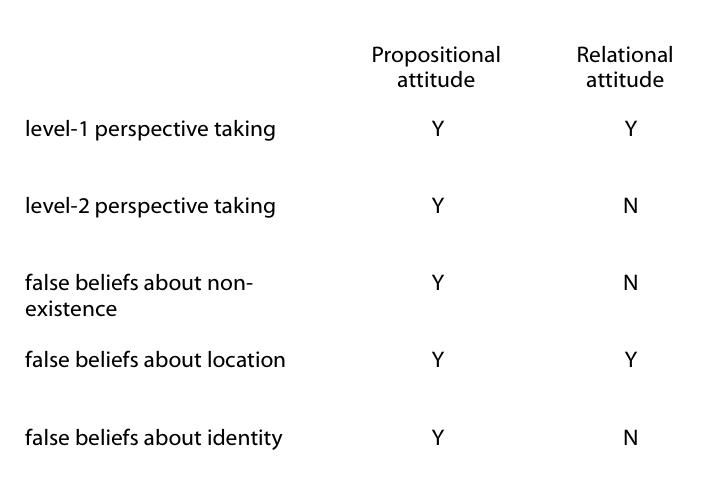
\includegraphics[width=0.25\textwidth]{fig/signature_limits_table.png}

\end{center}

\begin{center}

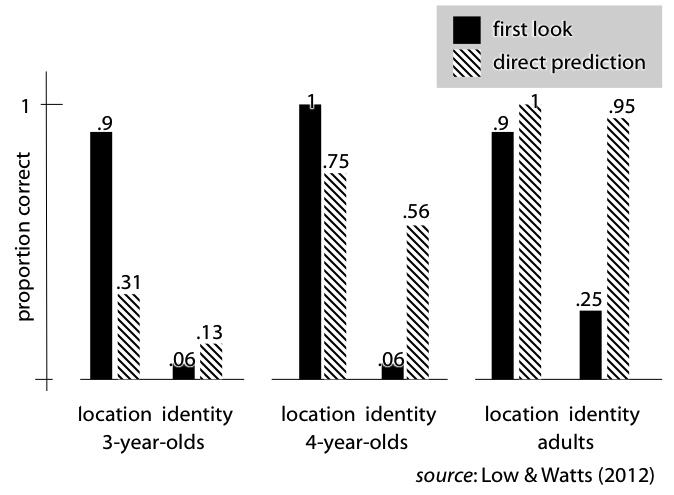
\includegraphics[width=0.3\textwidth]{fig/low_2012_fig.png}

\end{center}

For adults (and children who can do this),
representing perceptions and beliefs as such---and even merely holding in mind
what another believes, where no inference is required---involves a measurable
processing cost \citep{apperly:2008_back,apperly:2010_limits}, consumes attention
and working memory in fully competent adults \citealp{Apperly:2009cc,
lin:2010_reflexively, McKinnon:2007rr},  may require inhibition \citep{bull:2008_role}
and makes demands on executive function \citep{apperly:2004_frontal,samson:2005_seeing}.


\section{Objections}
‘the theoretical arguments offered [...] are [...] unconvincing, and [...]
the data can be explained in other terms’
(\citealp{carruthers:2015_two}; see also \citealp{carruthers:2015_mindreading}).

‘A cooperative multi-system architecture is better able to explain infant belief representation than a
parallel architecture, and causal representation, schemas and models provide a more promising basis
for flexible belief representation than does a rule-based approach of the kind described by Butterfill
and Apperly’ (\citealp{christensen:_twoa}; see also \citealp{michael:2016_flexible,michael:2013_mindreading}).

%--- end paste
%---------------

\footnotesize
\bibliography{$HOME/endnote/phd_biblio}

\end{multicols*}

\end{document}
